% ============================================================
%  Semaine 2 — HTML5 : structure & sémantique
%  Polycopié étudiant — cfpt·i | Anne Terrier
%  Charte graphique : charte cfpt·i originale, police sans-serif
% ============================================================
\documentclass[a4paper,11pt]{article}

\usepackage[T1]{fontenc}
\usepackage[utf8]{inputenc}
\usepackage[scaled=0.92]{helvet}
\renewcommand{\familydefault}{\sfdefault}
\usepackage[top=2.5cm, bottom=2.5cm, left=2.5cm, right=2.5cm, headheight=40pt]{geometry}
\usepackage{microtype}

\usepackage[dvipsnames,svgnames,table]{xcolor}
\usepackage{graphicx}
\usepackage{tikz}
\usetikzlibrary{positioning, shapes.geometric, arrows.meta, fit, backgrounds, decorations.pathreplacing}
\usepackage{booktabs}
\usepackage{tabularx}
\usepackage{array}
\usepackage{enumitem}
\usepackage[most]{tcolorbox}
\usepackage{fancyhdr}
\usepackage{lastpage}
\usepackage{titlesec}
\usepackage{listings}
\usepackage[hidelinks]{hyperref}

% ---------------------------------------------------------------
% Palette cfpt·i originale
% ---------------------------------------------------------------
\definecolor{cfptYellow}{HTML}{F5C400}
\definecolor{cfptBlack}{HTML}{1A1A1A}
\definecolor{cfptDarkGrey}{HTML}{555555}
\definecolor{cfptGrey}{HTML}{F2F2F2}
\definecolor{accentBlue}{HTML}{1D4E89}
\definecolor{lightBlue}{HTML}{D6E4F0}
\definecolor{codeGrey}{HTML}{F5F5F5}
\definecolor{successGreen}{HTML}{1E7145}
\definecolor{warningOrange}{HTML}{C55A11}

% Alias (le contenu du document utilise ces noms) vers la palette ci-dessus
\colorlet{uniInk}{cfptBlack}
\colorlet{uniNavy}{accentBlue}
\colorlet{uniTeal}{successGreen}
\colorlet{uniGold}{warningOrange}
\colorlet{uniGrey}{cfptDarkGrey}
\colorlet{uniPaper}{cfptGrey}
\colorlet{uniRule}{cfptDarkGrey!35}

\color{cfptBlack}

% --- En-tête / pied de page ---
\pagestyle{fancy}
\fancyhf{}
\renewcommand{\headrulewidth}{0pt}
\fancyhead[L]{\IfFileExists{Semaine2/images/cfpti.png}{
\includegraphics[height=18pt]{Semaine2/images/cfpti.png}}{\IfFileExists{cfpti.png}{
\includegraphics[height=18pt]{cfpti.png}}{}}}
\fancyhead[C]{\color{cfptDarkGrey}\small\textit{Développement Web --- Classe passerelle}}
\fancyhead[R]{\color{cfptDarkGrey}\small\textit{Semaine 2}}
\fancyfoot[L]{\color{cfptDarkGrey}\footnotesize Anne Terrier}
\fancyfoot[C]{\color{cfptDarkGrey}\footnotesize {HTML5 --- Structure \& sémantique}}
\fancyfoot[R]{\color{cfptDarkGrey}\footnotesize Page \thepage\ sur \pageref{LastPage}}
\renewcommand{\footrulewidth}{0.4pt}

% --- Titres sections : bandeau plein largeur ---
\newcommand{\sectionbox}[1]{%
  \colorbox{accentBlue}{%
    \parbox[c][1.6em][c]{\dimexpr\linewidth-2\fboxsep\relax}{%
      \color{white}\large\bfseries\hspace{4pt}\arabic{section}\qquad #1}}}

\newcommand{\sectionboxstar}[1]{%
  \colorbox{accentBlue}{%
    \parbox[c][1.6em][c]{\dimexpr\linewidth-2\fboxsep\relax}{%
      \color{white}\large\bfseries\hspace{4pt}#1}}}

\titleformat{\section}{\normalfont}{}{0pt}{\sectionbox}
\titleformat{name=\section,numberless}{\normalfont}{}{0pt}{\sectionboxstar}
\titleformat{\subsection}{\color{accentBlue}\normalsize\bfseries}{\rule[-.3ex]{3pt}{1.3em}}{6pt}{}
\titlespacing{\section}{0pt}{18pt}{8pt}
\titlespacing{\subsection}{0pt}{12pt}{4pt}

% --- supprime les retraits de paragraphe ---
\setlength{\parindent}{0pt}

% --- Listes ---
\setlist[itemize]{itemsep=3pt, topsep=4pt, parsep=0pt,
  leftmargin=1.4em, label={\color{cfptYellow}\textbullet}}
\setlist[itemize,2]{label={\color{cfptDarkGrey}--}, leftmargin=1.8em}
\setlist[enumerate]{itemsep=4pt, topsep=4pt, leftmargin=1.6em}

% --- Boîtes tcolorbox ---
\tcbset{
  definition/.style={
    colback=lightBlue!30, colframe=accentBlue,
    fonttitle=\bfseries\small\color{accentBlue},
    boxrule=0.8pt, arc=3pt,
    left=6pt, right=6pt, top=4pt, bottom=4pt,
    toptitle=2pt, bottomtitle=2pt},
  attention/.style={
    colback=cfptYellow!20, colframe=cfptYellow!80!black,
    fonttitle=\bfseries\small,
    boxrule=0.8pt, arc=3pt,
    left=6pt, right=6pt, top=4pt, bottom=4pt,
    toptitle=2pt, bottomtitle=2pt},
  astuce/.style={
    colback=successGreen!8, colframe=successGreen,
    fonttitle=\bfseries\small\color{successGreen},
    boxrule=0.8pt, arc=3pt,
    left=6pt, right=6pt, top=4pt, bottom=4pt,
    toptitle=2pt, bottomtitle=2pt},
  corrige/.style={
    colback=cfptGrey, colframe=cfptDarkGrey,
    fonttitle=\bfseries\small\color{cfptDarkGrey},
    boxrule=0.8pt, arc=3pt,
    left=6pt, right=6pt, top=4pt, bottom=4pt,
    toptitle=2pt, bottomtitle=2pt}
}

% --- Listings code ---
\lstset{
  basicstyle=\ttfamily\small,
  backgroundcolor=\color{codeGrey},
  frame=single, framerule=0.4pt,
  rulecolor=\color{cfptDarkGrey!40},
  breaklines=true,
  keywordstyle=\color{accentBlue}\bfseries,
  commentstyle=\color{cfptDarkGrey}\itshape,
  stringstyle=\color{successGreen},
  showstringspaces=false,
  numbers=left, numberstyle=\tiny\color{cfptDarkGrey},
  numbersep=8pt,
  captionpos=b,
}
\renewcommand{\lstlistingname}{Extrait}

% Coloration adaptée au HTML/CSS (balises)
\lstdefinelanguage{HTML5}{
  keywords={<!DOCTYPE, html, head, body, header, nav, main, section, article, aside, footer, h1, h2, h3, p, a, img, ul, ol, li, table, thead, tbody, tr, th, td, form, input, textarea, select, option, label, button, div, span, meta, title, link, script},
  sensitive=false,
  morecomment=[s]{<!--}{-->},
  morestring=[b]",
  keywordstyle=\color{accentBlue}\bfseries,
  stringstyle=\color{warningOrange},
  commentstyle=\color{cfptDarkGrey}\itshape,
}

\renewcommand{\arraystretch}{1.3}

% ============================================================
\begin{document}
% ============================================================

% --- Bandeau titre ---
\begin{tcolorbox}[
  colback=accentBlue, colframe=accentBlue,
  arc=4pt, left=12pt, right=12pt, top=10pt, bottom=10pt]
  \begin{minipage}{0.72\linewidth}
    {\color{white}\Large\bfseries Semaine 2}\\[4pt]
    {\color{white}\Large\bfseries HTML5 --- Structure \& sémantique}\\[4pt]
    {\color{lightBlue}\normalsize Anne Terrier --- Développement web, classe passerelle}
  \end{minipage}
  \hfill
  \begin{minipage}{0.22\linewidth}
    \raggedleft
    \begin{tabular}{rl}
      \multicolumn{2}{r}{\color{white}\small \today} \\
      \color{lightBlue}\small Cours & \color{white}\small 4h \\
      \color{lightBlue}\small TP    & \color{white}\small 4h \\
    \end{tabular}
  \end{minipage}
\end{tcolorbox}

\vspace{6pt}
\begin{tcolorbox}[definition, title={Objectifs de la semaine}]
\begin{itemize}
  \item Écrire une page HTML5 valide et sémantique
  \item Structurer le contenu avec les éléments appropriés
  \item Maîtriser le texte, les liens, les images, les listes et les tableaux
  \item Créer des formulaires fonctionnels avec les types d'\texttt{input} HTML5
  \item Prendre en compte les bases de l'accessibilité
\end{itemize}
\end{tcolorbox}

% ============================================================
\section{Qu'est-ce que le HTML ?}
% ============================================================

En semaine 1, nous avons vu que trois langages coexistent dans le navigateur. Le premier d'entre eux, le \textbf{HTML} (\textit{HyperText Markup Language}), est le langage qui décrit la \textbf{structure} et le \textbf{contenu} d'une page web. Pour créer une page web, il suffit de créer un fichier avec l'extension \textbf{.html}.

\begin{tcolorbox}[definition, title={Définition --- Langage de balisage}]
Le HTML n'est pas un langage de programmation : c'est un \textbf{langage de balisage}. On \textit{balise} le contenu à l'aide d'éléments (\textit{balises}) pour indiquer au navigateur ce que chaque morceau représente : un titre, un paragraphe, une image, un lien\dots
\end{tcolorbox}

\subsection{Anatomie d'une balise}

La plupart des éléments HTML fonctionnent par \textbf{paires} : une balise ouvrante et une balise fermante, qui encadrent un contenu.

\vspace{6pt}
\begin{center}
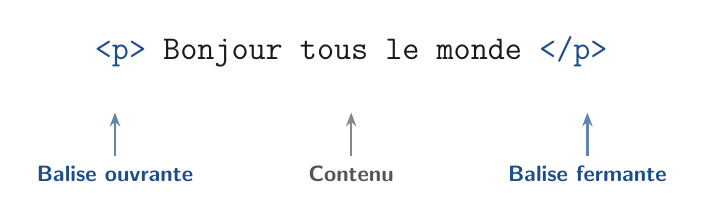
\begin{tikzpicture}[font=\small]
  \node[font=\ttfamily\large] (code) {%
    \textcolor{accentBlue}{<p>}%
    \textcolor{cfptBlack}{~Bonjour tous le monde~}%
    \textcolor{accentBlue}{</p>}};

  \node[below=1cm of code, xshift=-3.0cm,
        text=accentBlue, font=\footnotesize\bfseries] (lo) {Balise ouvrante};
  \node[below=1cm of code, xshift=0cm,
        text=cfptDarkGrey, font=\footnotesize\bfseries] (ct) {Contenu};
  \node[below=1cm of code, xshift=3.0cm,
        text=accentBlue, font=\footnotesize\bfseries] (lf) {Balise fermante};

  \draw[-{Stealth[length=5pt]}, accentBlue!70, thick] (lo.north) -- ++(0,0.55);
  \draw[-{Stealth[length=5pt]}, cfptDarkGrey!70, thick] (ct.north) -- ++(0,0.55);
  \draw[-{Stealth[length=5pt]}, accentBlue!70, thick] (lf.north) -- ++(0,0.55);
\end{tikzpicture}
\end{center}
\vspace{4pt}

Certaines balises sont \textbf{auto-fermantes} : elles n'encadrent aucun contenu et s'écrivent seules, comme \texttt{<img>} (une image) ou \texttt{<br>} (un retour à la ligne).

\subsection{Les attributs}

Une balise peut porter des \textbf{attributs} qui précisent son comportement ou ses propriétés. Un attribut s'écrit dans la balise ouvrante, sous la forme \texttt{nom="valeur"}.

\begin{lstlisting}[language=HTML5, caption={Un lien avec l'attribut href}]
<a href="https://www.hepia.ch">Site de la hepia</a>
\end{lstlisting}

Ici, \texttt{href} est l'attribut qui indique la destination du lien.

% ============================================================
\section{La structure d'un document HTML5}
% ============================================================

Toute page HTML5 suit le même squelette de base. Le voici, à connaître par cœur :

\begin{lstlisting}[language=HTML5, caption={Squelette minimal d'une page HTML5}]
<!DOCTYPE html>
<html lang="fr">
<head>
  <meta charset="UTF-8">
  <meta name="viewport" content="width=device-width, initial-scale=1.0">
  <title>Titre de la page</title>
</head>
<body>
  <!-- Le contenu visible de la page va ici -->
</body>
</html>
\end{lstlisting}

\begin{center}
\renewcommand{\arraystretch}{1.2}
\begin{tabularx}{\linewidth}{p{3.3cm}X}
  \toprule
  \rowcolor{uniNavy}
  \color{white}\textbf{Élément} & \color{white}\textbf{Rôle} \\
  \midrule
  \rowcolor{uniPaper}
  \texttt{<!DOCTYPE html>} & Indique au navigateur qu'il s'agit d'un document HTML5 \\
  \texttt{<html lang="fr">} & La racine du document ; \texttt{lang} précise la langue \\
  \rowcolor{uniPaper}
  \texttt{<head>} & Métadonnées invisibles : encodage, titre, feuilles de style\dots \\
  \texttt{<meta charset>} & Définit l'encodage des caractères (toujours \texttt{UTF-8}) \\
  \rowcolor{uniPaper}
  \texttt{<title>} & Le titre affiché dans l'onglet du navigateur \\
  \texttt{<body>} & Tout le contenu \textbf{visible} de la page \\
  \bottomrule
\end{tabularx}
\end{center}

\begin{tcolorbox}[attention, title={Important --- head vs body}]
Tout ce qui doit être \textbf{vu} par le visiteur va dans le \texttt{<body>}. Le \texttt{<head>} ne contient que des informations \textit{sur} la page (son titre, son encodage), jamais du contenu affiché.
\end{tcolorbox}

% ============================================================
\section{Les éléments sémantiques}
% ============================================================

Avant HTML5, les pages étaient construites avec des \texttt{<div>} partout. HTML5 a introduit des balises \textbf{sémantiques} : elles décrivent le \textit{rôle} de chaque zone de la page, ce qui la rend plus lisible pour les développeurs, les moteurs de recherche et les outils d'accessibilité.

\vspace{6pt}
\begin{center}
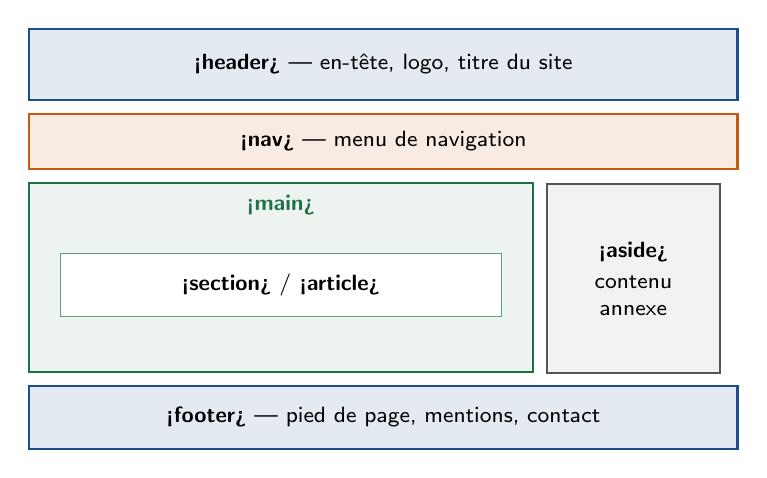
\begin{tikzpicture}[font=\footnotesize, every node/.style={align=center}]
  % header
  \node[draw=accentBlue, fill=accentBlue!12, thick, minimum width=9cm, minimum height=0.9cm] (header) {\textbf{<header>} --- en-tête, logo, titre du site};
  % nav
  \node[draw=warningOrange, fill=warningOrange!12, thick, minimum width=9cm, minimum height=0.7cm, below=0.15cm of header] (nav) {\textbf{<nav>} --- menu de navigation};
  % main container
  \node[draw=successGreen, fill=successGreen!8, thick, minimum width=6.4cm, minimum height=2.4cm, below=0.15cm of nav, xshift=-1.3cm, anchor=north] (main) {};
  \node[text=successGreen, font=\footnotesize\bfseries] at ([yshift=-0.3cm]main.north) {<main>};
  \node[draw=successGreen!70, fill=white, minimum width=5.6cm, minimum height=0.8cm] at ([yshift=-0.1cm]main.center) {\textbf{<section>} / \textbf{<article>}};
  % aside
  \node[draw=cfptDarkGrey, fill=cfptGrey, thick, minimum width=2.2cm, minimum height=2.4cm, right=0.15cm of main, anchor=north west, yshift=1.2cm] (aside) {\textbf{<aside>}\\[2pt]\footnotesize contenu\\annexe};
  % footer
  \node[draw=accentBlue, fill=accentBlue!12, thick, minimum width=9cm, minimum height=0.8cm, below=0.15cm of main, xshift=1.3cm] (footer) {\textbf{<footer>} --- pied de page, mentions, contact};
\end{tikzpicture}
\end{center}
\vspace{4pt}

\begin{center}
\renewcommand{\arraystretch}{1.2}
\begin{tabularx}{\linewidth}{p{2.6cm}X}
  \toprule
  \rowcolor{uniNavy}
  \color{white}\textbf{Balise} & \color{white}\textbf{Utilisation} \\
  \midrule
  \rowcolor{uniPaper}
  \texttt{<header>} & En-tête de la page ou d'une section (titre, logo) \\
  \texttt{<nav>} & Zone de navigation (menu principal, liens internes) \\
  \rowcolor{uniPaper}
  \texttt{<main>} & Le contenu principal, unique dans la page \\
  \texttt{<section>} & Un regroupement thématique de contenu \\
  \rowcolor{uniPaper}
  \texttt{<article>} & Un contenu autonome (un message du forum, un billet) \\
  \texttt{<aside>} & Un contenu annexe (barre latérale, encadré) \\
  \rowcolor{uniPaper}
  \texttt{<footer>} & Pied de page (mentions, contact, copyright) \\
  \bottomrule
\end{tabularx}
\end{center}

\begin{tcolorbox}[astuce, title={Section ou article ?}]
Retiens la règle simple : un \texttt{<article>} a du sens \textbf{tout seul}, sorti de son contexte (par exemple un message de forum que l'on pourrait citer ailleurs). Une \texttt{<section>} regroupe des contenus liés par un \textbf{thème} au sein de la page.
\end{tcolorbox}

% ============================================================
\section{Texte, liens et images}
% ============================================================

\subsection{Structurer le texte}

\begin{lstlisting}[language=HTML5, caption={Titres et paragraphes}]
<h1>Titre principal (un seul par page)</h1>
<h2>Sous-titre de niveau 2</h2>
<h3>Sous-titre de niveau 3</h3>

<p>Un paragraphe de texte. On peut y mettre du
   <strong>texte important</strong> ou de
   l'<em>emphase</em>.</p>
\end{lstlisting}

\begin{tcolorbox}[attention, title={Hiérarchie des titres}]
Les titres vont de \texttt{<h1>} à \texttt{<h6>}. Il ne faut en utiliser \textbf{qu'un seul \texttt{<h1>}} par page, et ne pas sauter de niveau (ne pas passer d'un \texttt{<h2>} directement à un \texttt{<h4>}). Cette hiérarchie est essentielle pour l'accessibilité et le référencement.
\end{tcolorbox}

\subsection{Les liens}

Le lien hypertexte, cœur du web, se crée avec la balise \texttt{<a>} et son attribut \texttt{href} :

\begin{lstlisting}[language=HTML5, caption={Différents types de liens}]
<!-- Lien externe -->
<a href="https://www.hepia.ch">Site de la hepia</a>

<!-- Lien vers une autre page du site -->
<a href="contact.html">Nous contacter</a>

<!-- Lien ouvrant un nouvel onglet -->
<a href="https://moodle.org" target="_blank">Moodle</a>

<!-- Lien interne : vers un element de la meme page -->
<a href="#contact">Aller au formulaire</a>
\end{lstlisting}

Ce dernier exemple, le \textbf{lien interne}, mérite qu'on s'y arrête : le \texttt{\#contact} ne pointe pas vers un fichier, mais vers un \textbf{élément de la page même} --- celui qui porte l'identifiant \texttt{contact}. Pour comprendre comment, il faut découvrir l'attribut \texttt{id}.

\subsection{L'attribut \texttt{id} : identifier un élément}

L'attribut \texttt{id} donne un \textbf{nom unique} à un élément de la page. On peut ensuite « pointer » vers cet élément.

\begin{lstlisting}[language=HTML5, caption={Un id sert de cible à un lien interne}]
<!-- Le lien pointe vers l'element d'id "contact" -->
<a href="#contact">Aller au formulaire</a>

<!-- ... plus bas dans la page ... -->
<section id="contact">
  <h2>Nous contacter</h2>
</section>
\end{lstlisting}

Cliquer sur le lien fait \textbf{défiler} la page jusqu'à la section \texttt{contact}. Le \texttt{\#} dans le \texttt{href} signifie « un élément de cette page », suivi de l'\texttt{id} visé.

\begin{tcolorbox}[attention, title={Règle d'or --- un id est unique}]
Sur une même page, \textbf{deux éléments ne peuvent jamais partager le même \texttt{id}}. C'est ce qui garantit qu'un \texttt{id} désigne un élément, et un seul. (À la différence de l'attribut \texttt{class}, que nous verrons avec le CSS, et qui peut, lui, être partagé.)
\end{tcolorbox}

\begin{tcolorbox}[astuce, title={L'id, un point d'accroche pour toute la suite}]
L'\texttt{id} ne sert pas qu'aux liens internes. C'est un \textbf{point d'accroche} vers un élément, réutilisé partout ensuite : il relie déjà un \texttt{<label>} à son champ (via \texttt{for}), il permettra de cibler un élément en \textbf{CSS} (semaine 3), et de le manipuler en \textbf{JavaScript} --- souviens-toi du tout premier exemple : \texttt{document.getElementById('btn')} allait chercher le bouton par son \texttt{id}.
\end{tcolorbox}

\subsection{Les images}

La balise \texttt{<img>} est auto-fermante. Elle a deux attributs importants :

\begin{lstlisting}[language=HTML5, caption={Insérer une image}]
<img src="logo.png" alt="Logo du MiniForum">
\end{lstlisting}

\begin{center}
\renewcommand{\arraystretch}{1.2}
\begin{tabularx}{\linewidth}{p{2cm}X}
  \toprule
  \rowcolor{uniNavy}
  \color{white}\textbf{Attribut} & \color{white}\textbf{Rôle} \\
  \midrule
  \rowcolor{uniPaper}
  \texttt{src} & Le chemin vers le fichier image (\textit{source}) \\
  \texttt{alt} & Un texte alternatif décrivant l'image \\
  \bottomrule
\end{tabularx}
\end{center}

\begin{tcolorbox}[attention, title={L'attribut alt n'est pas optionnel}]
Le texte \texttt{alt} est lu à voix haute par les lecteurs d'écran pour les personnes malvoyantes, et s'affiche si l'image ne charge pas. Il est \textbf{obligatoire} pour une page accessible. Décris ce que montre l'image, pas « image de\dots ».
\end{tcolorbox}

% ============================================================
\section{Listes et tableaux}
% ============================================================

\subsection{Les listes}

Il existe deux types de listes courantes :

\begin{lstlisting}[language=HTML5, caption={Liste non ordonnée et liste ordonnée}]
<!-- Liste a puces (unordered list) -->
<ul>
  <li>HTML</li>
  <li>CSS</li>
  <li>JavaScript</li>
</ul>

<!-- Liste numerotee (ordered list) -->
<ol>
  <li>Ouvrir le terminal</li>
  <li>Taper la commande</li>
  <li>Valider</li>
</ol>
\end{lstlisting}

\begin{tcolorbox}[astuce, title={Le bon usage}]
Utilise une liste \textbf{ordonnée} (\texttt{<ol>}) quand l'ordre compte (des étapes à suivre), et une liste \textbf{non ordonnée} (\texttt{<ul>}) quand l'ordre est indifférent (une liste de fonctionnalités).
\end{tcolorbox}

\subsection{Les tableaux}

Un tableau se construit ligne par ligne (\texttt{<tr>}), avec des cellules d'en-tête (\texttt{<th>}) et des cellules de données (\texttt{<td>}).

\begin{lstlisting}[language=HTML5, caption={Un tableau simple}]
<table>
  <thead>
    <tr>
      <th>Sujet</th>
      <th>Auteur</th>
    </tr>
  </thead>
  <tbody>
    <tr>
      <td>Bienvenue</td>
      <td>Alice</td>
    </tr>
  </tbody>
</table>
\end{lstlisting}

\paragraph{Fusionner des cellules}

Il arrive qu'une cellule doive s'étendre sur plusieurs colonnes ou plusieurs lignes. On utilise alors les attributs \texttt{colspan} (fusion horizontale) et \texttt{rowspan} (fusion verticale).

\begin{lstlisting}[language=HTML5, caption={Fusion de cellules avec colspan}]
<table>
  <tr>
    <th colspan="2">Coordonnees</th>
  </tr>
  <tr>
    <td>Email</td>
    <td>alice@exemple.ch</td>
  </tr>
</table>
\end{lstlisting}

Ici, la cellule d'en-tête « Coordonnees » occupe la largeur de \textbf{deux} colonnes grâce à \texttt{colspan="2"}. L'attribut \texttt{rowspan="2"} produirait le même effet sur la hauteur, en fusionnant deux lignes.

\begin{tcolorbox}[attention, title={Les tableaux, c'est pour des données}]
Un tableau HTML sert à présenter des \textbf{données tabulaires} (un planning, des résultats). Il ne faut \textbf{jamais} l'utiliser pour mettre en page une interface : c'est le rôle du CSS, que nous verrons en semaine 3.
\end{tcolorbox}

% ============================================================
\section{Les formulaires}
% ============================================================

Les formulaires permettent à l'utilisateur de \textbf{saisir} des informations : c'est ce qui rendra le MiniForum interactif. La balise conteneur est \texttt{<form>}.

\subsection{Le champ de saisie : \texttt{<input>}}

La balise \texttt{<input>} change de comportement selon son attribut \texttt{type}. HTML5 en propose de nombreux, avec validation automatique :

\begin{center}
\renewcommand{\arraystretch}{1.2}
\begin{tabularx}{\linewidth}{p{3.2cm}X}
  \toprule
  \rowcolor{uniNavy}
  \color{white}\textbf{type} & \color{white}\textbf{Usage} \\
  \midrule
  \rowcolor{uniPaper}
  \texttt{text} & Texte libre sur une ligne \\
  \texttt{email} & Adresse e-mail (validée automatiquement) \\
  \rowcolor{uniPaper}
  \texttt{password} & Mot de passe (caractères masqués) \\
  \texttt{number} & Valeur numérique \\
  \rowcolor{uniPaper}
  \texttt{checkbox} & Case à cocher \\
  \texttt{radio} & Bouton radio (choix unique) \\
  \bottomrule
\end{tabularx}
\end{center}

\subsection{Cases à cocher et boutons radio}

Ces deux types méritent un mot, car leur usage est un peu particulier. Une \textbf{case à cocher} (\texttt{checkbox}) permet plusieurs sélections indépendantes ; un \textbf{bouton radio} (\texttt{radio}) impose un choix \textbf{unique} parmi plusieurs.

\begin{lstlisting}[language=HTML5, caption={Cases à cocher et boutons radio}]
<!-- Cases a cocher : plusieurs choix possibles -->
<input type="checkbox" id="news" name="news">
<label for="news">Recevoir la newsletter</label>

<!-- Boutons radio : un seul choix (meme name !) -->
<input type="radio" id="pub" name="visibilite" value="public">
<label for="pub">Public</label>
<input type="radio" id="priv" name="visibilite" value="prive">
<label for="priv">Prive</label>
\end{lstlisting}

\begin{tcolorbox}[attention, title={La règle des boutons radio}]
Pour que des boutons radio fonctionnent comme un groupe (un seul sélectionnable à la fois), ils doivent \textbf{partager le même attribut \texttt{name}}. C'est cet attribut commun qui les relie ; l'attribut \texttt{value} distingue, lui, l'option choisie.
\end{tcolorbox}

\subsection{Un formulaire complet}

\begin{lstlisting}[language=HTML5, caption={Formulaire d'ajout de message}]
<form>
  <label for="pseudo">Votre pseudo :</label>
  <input type="text" id="pseudo" name="pseudo"
         placeholder="ex : alice" required>

  <label for="message">Votre message :</label>
  <textarea id="message" name="message"
            maxlength="500" required></textarea>

  <label for="categorie">Categorie :</label>
  <select id="categorie" name="categorie">
    <option value="general">General</option>
    <option value="aide">Aide</option>
  </select>

  <button type="submit">Envoyer</button>
</form>
\end{lstlisting}

\begin{center}
\renewcommand{\arraystretch}{1.2}
\begin{tabularx}{\linewidth}{p{2.6cm}X}
  \toprule
  \rowcolor{uniNavy}
  \color{white}\textbf{Élément} & \color{white}\textbf{Rôle} \\
  \midrule
  \rowcolor{uniPaper}
  \texttt{<label>} & L'étiquette décrivant un champ \\
  \texttt{<input>} & Un champ de saisie (selon son \texttt{type}) \\
  \rowcolor{uniPaper}
  \texttt{<textarea>} & Une zone de texte multi-lignes \\
  \texttt{<select>} & Une liste déroulante de choix \\
  \rowcolor{uniPaper}
  \texttt{<button>} & Un bouton (ici, pour envoyer le formulaire) \\
  \bottomrule
\end{tabularx}
\end{center}

\begin{tcolorbox}[attention, title={Le lien label / input}]
L'attribut \texttt{for} du \texttt{<label>} doit correspondre à l'\texttt{id} de l'\texttt{<input>} associé. Ce lien permet de cliquer sur l'étiquette pour activer le champ, et il est indispensable pour l'accessibilité.
\end{tcolorbox}

\subsection{Rendre un formulaire plus fiable}

On peut guider l'utilisateur et éviter les saisies erronées grâce à quelques attributs, sans écrire une seule ligne de JavaScript.

\begin{center}
\renewcommand{\arraystretch}{1.2}
\begin{tabularx}{\linewidth}{p{3cm}X}
  \toprule
  \rowcolor{uniNavy}
  \color{white}\textbf{Attribut} & \color{white}\textbf{Effet} \\
  \midrule
  \rowcolor{uniPaper}
  \texttt{placeholder} & Affiche un texte d'exemple grisé dans le champ vide \\
  \texttt{required} & Rend le champ obligatoire : le formulaire refuse de partir s'il est vide \\
  \rowcolor{uniPaper}
  \texttt{maxlength} & Limite le nombre de caractères saisissables \\
  \texttt{min} / \texttt{max} & Bornent une valeur numérique (avec \texttt{type="number"}) \\
  \bottomrule
\end{tabularx}
\end{center}

\begin{tcolorbox}[astuce, title={La validation HTML5, gratuite et automatique}]
Le navigateur vérifie \textbf{lui-même} certains champs avant l'envoi : un \texttt{type="email"} refuse une adresse mal formée, un champ \texttt{required} vide bloque l'envoi. Cette \textbf{validation HTML5} est immédiate, sans JavaScript, et améliore nettement l'expérience utilisateur. Nous la compléterons plus tard côté serveur, car une validation côté navigateur ne suffit jamais à elle seule pour la sécurité.
\end{tcolorbox}

\begin{tcolorbox}[definition, title={Et l'envoi des données ?}]
Tu as sans doute remarqué que ce formulaire ne va, pour l'instant, \textbf{nulle part} : cliquer sur « Envoyer » ne fait rien de visible. C'est normal. L'envoi réel des données vers un \textbf{serveur} (via les attributs \texttt{action} et \texttt{method} de la balise \texttt{<form>}) sera vu en \textbf{phase 3}, quand le MiniForum aura un serveur Node.js pour les recevoir.
\end{tcolorbox}

% ============================================================
\section{Accessibilité : les bons réflexes}
% ============================================================

L'\textbf{accessibilité} consiste à rendre les pages utilisables par tous, y compris les personnes en situation de handicap (malvoyance, navigation au clavier\dots). Dès la semaine 2, quelques réflexes simples font une grande différence :

\begin{itemize}
  \item Toujours renseigner l'attribut \texttt{alt} des images.
  \item Respecter la hiérarchie des titres (\texttt{<h1>} puis \texttt{<h2>}\dots sans sauter de niveau).
  \item Associer chaque \texttt{<input>} à un \texttt{<label>} via \texttt{for} / \texttt{id}.
  \item Utiliser les balises sémantiques (\texttt{<nav>}, \texttt{<main>}\dots) plutôt que des \texttt{<div>} génériques.
  \item Préciser la langue de la page avec \texttt{<html lang="fr">}.
\end{itemize}

\begin{tcolorbox}[astuce, title={Valider son code}]
Le service en ligne \textbf{validator.w3.org} vérifie qu'une page HTML est correctement écrite (balises bien fermées, structure valide). Prends l'habitude de valider ton code : un HTML valide est la base d'un site fiable.
\end{tcolorbox}

% ============================================================
\section{Lexique de la semaine}
% ============================================================

\begin{center}
\renewcommand{\arraystretch}{1.0}
\begin{tabularx}{\linewidth}{p{4cm}X}
  \toprule
  \rowcolor{uniNavy}
  \color{white}\textbf{Terme} & \color{white}\textbf{Définition} \\
  \midrule
  \rowcolor{uniPaper}
  Balise (\textit{tag}) & Élément HTML qui décrit un morceau de contenu \\
  Attribut & Information complémentaire placée dans une balise (\texttt{nom="valeur"}) \\
  \rowcolor{uniPaper}
  Sémantique & Choix d'une balise selon le \textit{sens} du contenu, pas son apparence \\
  Élément auto-fermant & Balise sans contenu ni fermeture (\texttt{<img>}, \texttt{<br>}) \\
  \rowcolor{uniPaper}
  \texttt{id} & Identifiant \textbf{unique} d'un élément ; cible d'un lien interne, d'un label, du CSS et du JS \\
  \texttt{<head>} & Zone des métadonnées, invisible pour le visiteur \\
  \rowcolor{uniPaper}
  \texttt{<body>} & Zone du contenu visible de la page \\
  Accessibilité & Ensemble des pratiques rendant une page utilisable par tous \\
  \rowcolor{uniPaper}
  \texttt{alt} & Texte alternatif décrivant une image \\
  Formulaire & Ensemble de champs permettant à l'utilisateur de saisir des données \\
  \rowcolor{uniPaper}
  \texttt{required} & Attribut rendant un champ obligatoire avant l'envoi \\
  Validation HTML5 & Vérification automatique des champs par le navigateur, sans JavaScript \\
  \bottomrule
\end{tabularx}
\end{center}

% ============================================================
\section*{Pour aller plus loin}
% ============================================================

\begin{tcolorbox}[astuce, title={Quiz et travaux pratiques}]
\begin{itemize}
  \item Un \textbf{quiz d'auto-évaluation} sur cette semaine est disponible sur Moodle.
  \item La \textbf{fiche TP} (squelette HTML du MiniForum) est distribuée séparément : \textit{S02\_TP.pdf}.
\end{itemize}
\end{tcolorbox}

% ============================================================
\section*{Résumé de la semaine}
% ============================================================

\begin{tcolorbox}[definition, title={Ce qu'il faut retenir}]
\begin{itemize}
  \item Le HTML est un langage de \textbf{balisage} qui décrit la structure du contenu
  \item Toute page suit le même squelette : \texttt{<!DOCTYPE>}, \texttt{<head>}, \texttt{<body>}
  \item Les balises \textbf{sémantiques} (\texttt{<header>}, \texttt{<nav>}, \texttt{<main>}, \texttt{<article>}, \texttt{<footer>}) décrivent le rôle de chaque zone
  \item On structure le texte avec les titres \texttt{<h1>}\dots\texttt{<h6>}, les liens \texttt{<a>}, les images \texttt{<img>}
  \item Les \textbf{formulaires} (\texttt{<form>}, \texttt{<input>}, \texttt{<label>}) permettent la saisie de données
  \item L'\textbf{accessibilité} se construit dès le HTML : \texttt{alt}, \texttt{label}, hiérarchie des titres
\end{itemize}
\end{tcolorbox}

\vspace{8pt}
\begin{tcolorbox}[attention, title={Pour la semaine 3}]
\begin{itemize}
  \item Avoir terminé le squelette HTML du MiniForum (en-tête, liste de sujets, formulaire)
  \item Vérifier que sa page passe le validateur \textbf{validator.w3.org} sans erreur
  \item La semaine 3 introduira le \textbf{CSS} pour donner du style à cette structure
\end{itemize}
\end{tcolorbox}

\end{document}
